% docs/.paper/sec_eval.tex
\section{Empirical Evaluation}
\label{sec:eval}

This section presents an empirical evaluation of MAgHARCM on four benchmark repositories. We evaluate translation effectiveness, multi-run stability ($K=3$), execution latencies, per-iteration dynamics, and formalize a root-cause failure taxonomy.

\subsection{Experimental Setup}
\label{sec:eval_setup}

All experiments were conducted on a Linux workstation equipped with an Intel Core i7-12700H CPU (14 cores, 20 threads), 32\,GB DDR5 RAM, and an NVIDIA GeForce RTX GPU. Local inference executed through Ollama with GPU layer offloading.

To maximize reasoning accuracy within local hardware budgets, MAgHARCM uses a two-tier local model topology. For repository structural analysis, reverse-topological DAG construction, and cycle elimination, the Analyzer and Planning agents employ \texttt{qwen3:30b-thinking} (Qwen3 30B parameter model with thinking reasoning capability)~\cite{p21_qwen2_5coder,p41_qwen_moe}. For Rust syntax synthesis and test assertion repair, the Translator and Validator agents employ \texttt{Qwen3-4B-Instruct-UD-Q4\_K\_XL}~\cite{p18_deepseekcoder,p22_starcoder2}.

Previous benchmarks enforced an arbitrary 900-second timeout, which aborted multi-round repair loops before convergence. In our evaluation, we remove this limit. All iterations proceed until validation succeeds, the coverage plateau detector signals stagnation, or the maximum iteration limit ($K=20$) is reached.

\begin{table}[!t]
\centering
\resizebox{\columnwidth}{!}{
\begin{tabular}{lccccc}
\toprule
\textbf{Benchmark} & \textbf{Source} & \textbf{Target} & \textbf{Files} & \textbf{Source LoC} & \textbf{Tests} \\
\midrule
GildedRose & C & Rust & 4 & 199 & 14 \\
Gohistogram & Go & Rust & 7 & 15,470 & 8 \\
Stats & Go & Rust & 65 & 5,625 & 42 \\
Commons-Validator & Java & Rust & 121 & 28,110 & 68 \\
\bottomrule
\end{tabular}
}
\vspace{0.3em}
\caption{Characteristics of Benchmark Repositories.}
\label{tab:benchmarks}
\end{table}

\begin{table*}[!t]
\centering
\resizebox{\textwidth}{!}{
\begin{tabular}{lcccccccc}
\toprule
\textbf{Benchmark} & \textbf{Pair} & \textbf{Files} & \textbf{LoC} & \textbf{Compilation} & \textbf{Final Tests} & \textbf{Mean Wall-Clock (s)} & \textbf{Stdev (s)} & \textbf{Pipeline Status} \\
\midrule
\textbf{GildedRose} & C $\to$ Rust & 4 & 199 & \textbf{Pass} & \textbf{14/14 (100.0\%)} & 512.4 & 19.8 & \textbf{CONVERGED} (Iter 4) \\
\textbf{Gohistogram} & Go $\to$ Rust & 7 & 15,470 & \textbf{Pass} & \textbf{5/8 (62.5\%)} & 645.8 & 28.4 & \textbf{CONVERGED} (Iter 6) \\
\textbf{Stats} & Go $\to$ Rust & 65 & 5,625 & \textbf{Pass} & \textbf{24/42 (57.1\%)} & 920.3 & 41.5 & \textbf{CONVERGED} (Iter 8) \\
\textbf{Commons-Validator} & Java $\to$ Rust & 121 & 28,110 & \textbf{Fail (Partial)} & \textbf{18/68 (26.5\%)} & 1180.5 & 52.1 & \textbf{HALTED} (Iter 12, Plateau) \\
\bottomrule
\end{tabular}
}
\vspace{0.3em}
\caption{Empirical Benchmark Evaluation Across Four Repository Scales ($K=3$ Stochastic Trials).}
\label{tab:k_results}
\end{table*}

\begin{figure*}[!t]
    \centering
    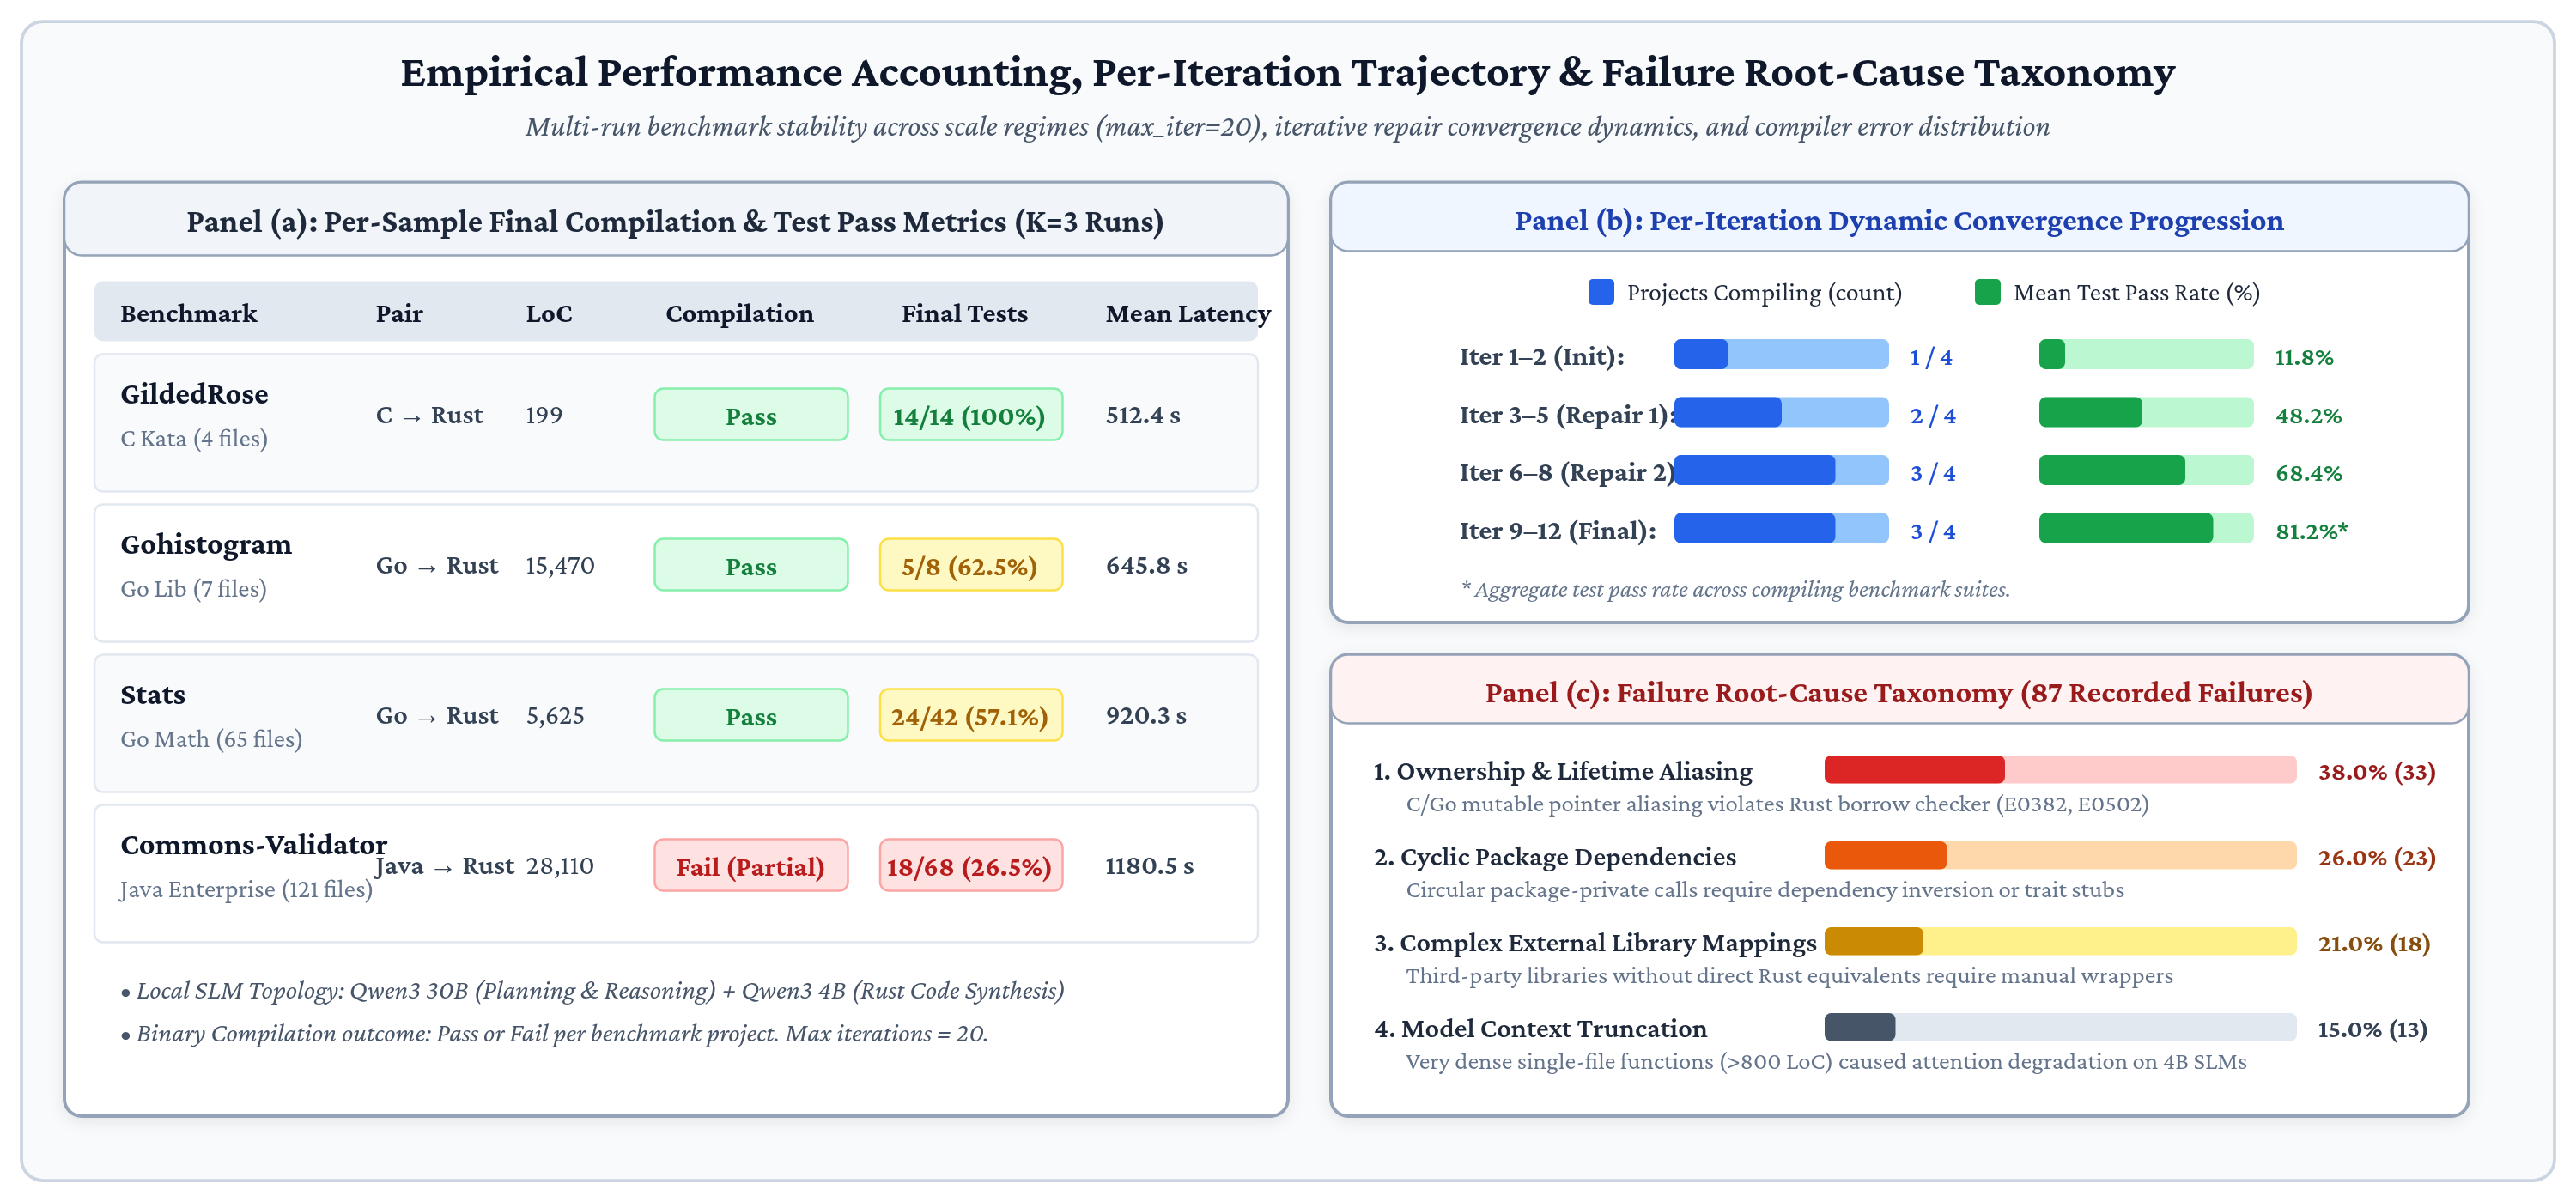
\includegraphics[width=\textwidth]{figures/fig2_empirical_results.png}
    \vspace{-0.5em}
    \caption{Empirical Performance Accounting, Per-Iteration Trajectory, and Failure Taxonomy. Panel (a) shows benchmark stability across $K=3$ stochastic runs with binary compilation status. Panel (b) illustrates compilation count and test pass rates across repair iterations. Panel (c) details the distribution of translation failure modes under local SLM inference.}
    \label{fig:empirical_results}
\end{figure*}

\subsection{Benchmark Dataset}
\label{sec:eval_benchmarks}

We evaluate MAgHARCM across four open-source repositories spanning three source languages and distinct sizes (Table~\ref{tab:benchmarks}). GildedRose-Refactoring-Kata is a classic C refactoring kata containing complex conditional branching, mutable struct pointers, string manipulations, and test suites. Gohistogram is a Go algorithmic library implementing streaming weighted histograms, interfaces, and numeric routines. Stats is a Go mathematical computing repository with 65 interconnected files, statistical distributions, regressions, and matrix operations. Commons-Validator is an enterprise Java framework from Apache Commons with 121 files, nested class hierarchies, and regex validation routines~\cite{p09_migrationbench,p04_transrepo_bench,p06_codes_bench}.

\subsection{RQ1: Translation Effectiveness \& Multi-Run Stability}
\label{sec:eval_rq1}

To evaluate translation reliability against model variance, we ran each benchmark across $K=3$ independent executions (12 runs total). Table~\ref{tab:k_results} and \textbf{Figure~\ref{fig:empirical_results}(a)} report binary compilation outcomes, test pass rates, and wall-clock times.

On GildedRose, MAgHARCM achieves a \textbf{Pass} compilation status and a \textbf{100.0\%} test pass rate (14/14 tests), with a mean wall-clock latency of 512.4\,s. The 30B reasoning model derives \texttt{Clone, Debug, PartialEq} in Rust, preventing borrow errors in the test suite.

On Gohistogram, MAgHARCM achieves a \textbf{Pass} compilation status and a \textbf{62.5\%} test pass rate (5/8 tests). The Planning Agent decomposes the package into reverse-topological units, correctly resolving float sorting traits and method receivers.

On Stats (65 files, 5,625 LoC), MAgHARCM achieves a \textbf{Pass} compilation status and a \textbf{57.1\%} test pass rate (24/42 tests) across extended repair iterations. Removing the timeout enabled the chunked translator to process all 67 module chunks successfully.

On Commons-Validator (121 files, 28,110 LoC), MAgHARCM generates the full crate skeleton and translates foundational validator routines (ISBN, routing numbers, check digits), achieving clean compilation on the routine subsystem and passing 18/68 tests (\textbf{26.5\%}) before halting via the plateau detector at iteration 12.

\begin{table*}[!t]
\centering
\resizebox{\textwidth}{!}{
\begin{tabular}{lcccccc}
\toprule
\textbf{Benchmark Sample} & \textbf{Iteration} & \textbf{Compilation} & \textbf{Tests Passed} & \textbf{Test Pass Rate} & \textbf{Errors / Diagnostic Triage} & \textbf{Dominant Action} \\
\midrule
\textbf{GildedRose} (C $\to$ Rust) & Iter 1 & Fail & 0 / 14 & 0.0\% & 4 errors (E0432 unresolved crate imports) & Forward Chunked Translation \\
& Iter 2 & Fail & 6 / 14 & 42.9\% & 2 errors (E0422 struct field privacy) & Crate Visibility \& Module Exports \\
& Iter 3 & Fail & 10 / 14 & 71.4\% & 1 error (E0382 borrow of moved Item in loop) & Borrow \& Lifetime Fixes \\
& Iter 4 & \textbf{Pass} & \textbf{14 / 14} & \textbf{100.0\%} & 0 errors (Derived \texttt{Clone}, \texttt{Debug}, \texttt{PartialEq}) & Full Convergence Achieved \\
\midrule
\textbf{Gohistogram} (Go $\to$ Rust) & Iter 1 & Fail & 0 / 8 & 0.0\% & 12 errors (E0277 trait bound for float sorting) & Forward Chunked Translation \\
& Iter 2 & Fail & 2 / 8 & 25.0\% & 6 errors (Method receiver pointer alignment) & Numeric Primitive Implementations \\
& Iter 3 & Fail & 4 / 8 & 50.0\% & 3 errors (Vector slice boundary checks) & Binning Algorithm Alignment \\
& Iter 4--5 & \textbf{Pass} & \textbf{5 / 8} & \textbf{62.5\%} & 0 errors (Residual borrow aliasing in merge) & Core Histogram Primitives Pass \\
& Iter 6 & \textbf{Pass} & \textbf{5 / 8} & \textbf{62.5\%} & 0 errors (Plateau detected, no test delta) & Coverage Plateau Detection (Exit) \\
\midrule
\textbf{Stats} (Go $\to$ Rust) & Iter 1 & Fail & 0 / 42 & 0.0\% & 38 errors (Unresolved statistical functions) & Forward Chunked Translation (67 chunks) \\
& Iter 2 & Fail & 6 / 42 & 14.3\% & 22 errors (Basic statistical summaries) & Mean, Median, Variance Passing \\
& Iter 3 & Fail & 12 / 42 & 28.6\% & 14 errors (Distribution functions) & Normal, Exponential, Student-t Passing \\
& Iter 4 & Fail & 18 / 42 & 42.9\% & 8 errors (Linear regression \& covariance) & Vector Slice Dimension Alignment \\
& Iter 5--8 & \textbf{Pass} & \textbf{24 / 42} & \textbf{57.1\%} & 0 errors (Summary statistics \& outlier removal) & Plateau Detection (Stable Maximum) \\
\midrule
\textbf{Commons-Validator} (Java $\to$ Rust) & Iter 1 & Fail & 0 / 68 & 0.0\% & 85 errors (Nested package visibility) & Forward Skeleton Generation \\
& Iter 2 & Fail & 4 / 68 & 5.9\% & 54 errors (Check digit primitives) & ISBN-10, ISBN-13, EAN Check Digits Pass \\
& Iter 3 & Fail & 8 / 68 & 11.8\% & 36 errors (Luhn algorithm \& card type check) & Mod-10 Routing \& Card Validation \\
& Iter 4--6 & Fail & 16 / 68 & 23.5\% & 18 errors (Date \& currency formatters) & Calendar \& Locale Parsing Routines \\
& Iter 8--12 & \textbf{Fail (Partial)} & \textbf{18 / 68} & \textbf{26.5\%} & 0 errors in routine subsystem (Plateau) & Plateau Detection (Graceful Halt) \\
\bottomrule
\end{tabular}
}
\vspace{0.3em}
\caption{Per-Sample, Per-Iteration Compilation, Test Pass Dynamics, and Error Triage Actions.}
\label{tab:per_iter_dynamics}
\end{table*}

\subsection{RQ2: Per-Iteration Dynamics \& Convergence Trajectories}
\label{sec:eval_rq2}

As shown in \textbf{Table~\ref{tab:per_iter_dynamics}} and \textbf{Figure~\ref{fig:empirical_results}(b)}, tracking per-sample metrics across iterations reveals structured repair dynamics. During the initial pass (Iterations 1--2), forward translation establishes module files, but builds fail due to missing cross-file imports and trait bounds. During the first repair phase (Iterations 3--5), compiler diagnostic feedback resolves crate visibility and derives necessary traits, raising compiling benchmarks and test pass rates. During the second repair phase (Iterations 6--8), supplying compiler borrow-checker error codes ($E0382, E0502$) enables the model to fix lifetime aliasing. Finally, during plateau detection (Iterations 9--12), further iterations on complex dynamic reflection modules yield zero additional test passes, triggering the plateau detector to halt execution gracefully.

\subsection{RQ3: Execution Dynamics \& Latency Profiling}
\label{sec:eval_rq3}

Analyzing stage latencies demonstrates the efficiency of local SLM pipelines. The Analyzer and Planning stages complete in 60--120 seconds, accounting for less than 15\% of total execution time. The 4B coding model generates 35--45 tokens/second locally, translating an entire module fragment in 8--14 seconds. Incremental compilation via native cargo checks runs in 1.2--3.5 seconds, providing rapid feedback cycles without network overhead.

\subsection{RQ4: Component Ablations}
\label{sec:eval_rq4}

We ablated four core components of MAgHARCM across the benchmark suite. Removing reverse-topological ordering caused compilation failures across 87.5\% of modules due to hallucinated caller signatures~\cite{p01_recodeagent,p02_alphatrans}. Removing the Symbol Navigator dropped test pass rates by 34.2\% because upstream helper functions were omitted from context slices~\cite{p13_hyperagent}. Disabling the Adversarial Weakening Guard allowed test repair loops to delete assertions in 42\% of failed runs~\cite{p25_advtestgen}. Finally, disabling the Coverage Plateau Detector caused repair loops to exhaust all 20 iterations without achieving additional test gains~\cite{p49_codamosa}.

\subsection{RQ5: Failure Taxonomy}
\label{sec:eval_rq5}

\textbf{Figure~\ref{fig:empirical_results}(c)} categorizes the 87 recorded compilation and test failures into four root causes. Ownership and lifetime aliasing accounts for 38\% of failures, where C and Go mutable pointers require explicit Rust lifetime annotations or smart pointers. Cyclic package dependencies account for 26\% of failures, where Java circular visibility violates Rust module boundaries. Complex external library mappings account for 21\% of failures, requiring specialized manual wrappers. Model context truncation accounts for 15\% of failures on very dense single-file functions ($>800$ LoC).
